% !TEX TS-program = pdflatex
% !TEX encoding = UTF-8 Unicode

% Compile with: pdflatex doski.tex \ bibtex doksi \ pdflatex doksi.tex
\documentclass[12pt]{article}
\usepackage[utf8]{inputenc}
\usepackage{float}

\usepackage{siunitx} % for microseconds
\usepackage{xcolor}
\usepackage{hyperref}
\hypersetup{
    colorlinks,
    linkcolor=black,
    citecolor=black,
    urlcolor={blue!80!black}
}
% 
\urlstyle{same}
\usepackage{appendix}
\usepackage[a4paper, width=170mm, top=25mm, bottom=25mm, bindingoffset=6mm]{geometry}
\usepackage{graphicx}
\graphicspath{ {../diagrams/}, {../time_diagrams/} }

%%% PACKAGES
\usepackage{booktabs} % for much better looking tables
\usepackage{array} % for better arrays (eg matrices) in maths
\usepackage{paralist} % very flexible & customisable lists (eg. enumerate/itemize, etc.)
\usepackage{verbatim} % adds environment for commenting out blocks of text & for better verbatim
\usepackage{subfig} % make it possible to include more than one captioned figure/table in a single float

\usepackage[magyar]{babel}
\usepackage{t1enc}

\setlength{\parindent}{0pt} % disable automatic indentation

% definition of tab command
\newcommand\tab[1][1cm]{\hspace*{#1}}

%%%%%%%%%%%%%%%%%%%%%%%%%%%%%%%%%%%%%%%%%%%%%%%%%%%%%%%%%%%%%%%%%%%%%%%%%%%%%%%%%%%%%%%%%%%%%%%%%%%%%%%%%%%%%%%%%%%%%%%%%%%%%%%

\title{Programozható LED-fűzéren alapuló reklámpanel \\
	LED fűzér vezérlése: adatok kiírása}
\author{Patka Zsolt-András \\ Számítástechnika BSc}
\date{2019.12.16}

\begin{document}
\maketitle
\pagenumbering{gobble}

\newpage
\tableofcontents
\newpage

\pagenumbering{arabic}
\section{Beveztő}
\tab A projekt célja egy LED-fűzér vezérlése és ennek segítségével egy reklámszöveg megjelenítése.
Ehhez egy Basys3 FPGA lap és egy Worldsemi WS2813 ledfűzér lesz felhasználva.

\section{Követelmények}
\subsection{Funkcionális követelmények}
\begin{itemize}
\item Lehetséges legyen egy reklámszöveget kiírni a ledfűzérek által létrehozott mátrix-ra.
\item Egy sorban minimum 100 LED található
\item Az egyes ledfűzérek szinkronba működjenek
\item A kiírás párhuzamosan történik az adott ledfűzéreken
\item Másodpercenként 60 frissítés (60 Hz)
\item Mozgó szöveg
\end{itemize}

\subsection{Nem funkcionális követelmények}
\begin{itemize}
\item Benti használatra van tervezve
\item Ha az FPGA-lapnak lesz készítve külön tokozat, akkor IP31-es standardnak kell megfeleljen
\item Ha az FPGA-lapnak nem lesz készítve külön tokozat, akkor nem felel meg IP standardnak (IP00)
\end{itemize}

\subsection{Fejlesztési követelmények}
\begin{itemize}
\item Implementáció VHDL nyelvben
\item Szimulációs állomány a rendszer tesztelésére
\item Adatok kiírása lehetséges a LED fűzérre
\item Modularitás
\begin{itemize}
	\item WS2813\_Driver: Egy 24 bit-es blokkot küldő modul
	\item WS2813\_Controller: Egy szálon több 24 bit-es blokkot kiküldő, a WS2813\_Driver modult fehasználó modul
	\item WS2813\_TopLevel: Több ledfűzérre való kiírást lehetővé tevő modul,
	
	 több WS2813\_Controller modul BRAM-al való összekötése által
\end{itemize}
\item Opcionális: 
\begin{itemize}
	\item Pár betű kódolása (3-4)
	\item Betük tárolása BRAM memóriában
\end{itemize}
\end{itemize}

\section{Rendszer-specifikáció}
\begin{itemize}
\item WS2813 egyszálú adatátvitel protokolljának helyes használata
\item Worldsemi WS2813 90 LED-es ledfűzér van felhasználva
\item Digilent Basys3 FPGA vezérli a ledfűzért 
\end{itemize}

\section{Tervezés}
\subsection{WS2813 egyszálú adatátvitel protokoll leírása}
\tab A LED-eket vezérlő áramkörök egymás után vannak bekötve úgy, hogy az egyik áramkörnek az adatkimenete a következő áramkörnek az adatbemenetét képzi.
Egyszálú az adatátvitel, fontos a protokoll betartása, ahhoz, hogy adatok tudjanak megjelenni a LED-fűzéren.

\tab Amikor egy áramkör megkap egy 24 bit-es kódot, akkor ezt addig tárolja amíg más kódot nem kap, vagy a tápforrást el nem veszti.

\subsubsection{A 24 bit-es kód}

\tab A 24 bit-es kód a következőképpen kell kinézzen: 

\tab \textbf{8 bit GREEN} | \textbf{8 bit RED} | \textbf{8 bit BLUE}

\tab Az adatátvitel a következő sorrendben kell történjen: 
\begin{enumerate}
\item GREEN
\item RED
\item BLUE
\end{enumerate}

\subsubsection{Bit-ek küldési sorrendje}

\tab Az egyes byte-ok küldését úgy kell elvégezni, hogy az \textbf{MSB}-vel kell kezdeni és haladni az \textbf{LSB} fele. 
24 bit-es kód részletesebb felbontása: 
\begin{itemize}
\item \textit{G7 G6 G5 G4 G3 G2 G1 G0 | R7 R6 R5 R4 R3 R2 R1 R0 | B7 B6 B5 B4 B3 B2 B1 B0}
\end{itemize}

\tab A küldés a következő sorrendben kell elvégződjön (balról jobbra): 
\begin{itemize}
\item \textbf{G7 G6 G5 G4 G3 G2 G1 G0 | R7 R6 R5 R4 R3 R2 R1 R0 | B7 B6 B5 B4 B3 B2 B1 B0}
\end{itemize}

\subsubsection{Időzítések}

\tab Minden 24 bit-es adatátvitel után kell legalább \SI{50}{\micro\second}-ot várakozni, alacsony feszűltségen. Ez jelzi azt, hogy egy 24 bit-es blokk továbbítása megtörtént.

\tab Az egyes bit-ek átvitele a következőképp történik:

\begin{itemize}
\item Logikai 1-es
	\begin{itemize}
	\item \SI{0.8}{\micro\second}-ot magas feszűltségen
	\item \SI{0.45}{\micro\second}-ot alacson feszűltségen
	\end{itemize}
\item Logikai 0-ás
	\begin{itemize}
	\item \SI{0.4}{\micro\second}-ot magas feszűltségen
	\item \SI{0.85}{\micro\second}-ot alacson feszűltségen
	\end{itemize}
\item 24 bit-es adatblokk küldése után: 
	\begin{itemize}
		\item $ > \SI{50}{\micro\second}$-ot alacsony feszűltségen
	\end{itemize}
\end{itemize}

\tab A bit-ek továbbításánál egy +/- \SI{150}{\nano\second}-os eltérés megengedett.

\tab A várakozási értékek nem az adatlapból, hanem egy útmutatóból\cite{neopixel2019adafruit} lettek kivéve. 
Az útmutató szerint az adatlapban levő értékek rosszul vannak kiszámolva.

\tab Ha az útmutatóban megadott értékek nem megfelelő működéshez vezetnek, akkor az adatlapban\cite{WS2813datasheet} levő értékek lesznek felhasználva. 
Ez a valós rendszeren levő tesztelés közben fog kiderülni.


\subsection{Véges állapotú adatútas automata}
\tab A fejlesztési követelményekben levő három modul implementációja a véges állapotú adatútas automata\cite{brassai2018ukda_auto} tervezési mintával lett kivitelezve.
Az adott tervezési minta egyszerűvé teszi a tervezést, mivel jól definiált lépéseken keresztül el lehet jutni egy működő tervhez.


\subsection{WS2813\_Driver tervezése}
Ez a modul felelős egy 24 bit-es blokk kiküldéséért 


\subsubsection{Elvégezendő RT műveletek azonosítása}

Az időzítések implementálásához egy számláló lesz használva. A 100 MHz-es órajel ami fel lesz használva időben $\SI{0.01}{\micro\second}$-nak felel meg. 
Így a szükséges ciklusok száma (amennyit várakoztatni kell bizonyos feszűltségszinten, ahhoz, hogy a WS2813 protokollja be legyen tartva) egész.
Ebből már látható, hogy definiálható két művelet: $i \Leftarrow ciklus\_szam$, $i \Leftarrow i - 1$ (ahol i a számláló).

\indent Az egyszerűség kedvéért, egy belső regiszternek, amely a színadatokat tartalmazza (\textbf{data}), mindig a 24. bitje kerül kiküldésre.
Tehát minden bit kiküldése után ennek a regiszternek az értékeit el kell csúsztatni (shift-elni) egyet balra: $data \Leftarrow data << 1$

\indent Egy 24-bites blokk kiküldése után kell küldeni egy "RES" jelet, vagyis több ideig alacsony feszűltségen kell tartani a kimenetet. 
Ehhez számolni kell a már elküldött bitek számát $bit\_count \Leftarrow bit\_count - 1$, ahol bit\_count az eddig elküldött bitek számát tartalmazza.
Az elküldött bit-ek 23-től számolódnak lefele, mivel a nullához való hasonlítás hatékonyabb, mint egy adott értékhez való hasonlítás.

\subsubsection{Adatfüggőségek identifikálása}

Mivel nagyon egyszerű RT műveletekkel meg lehet oldani az adott feladatot, nem merűlnek fel adatfüggőségek.

\subsubsection{Célregiszterek azonosítása}

Szükséges regiszterek:
\begin{itemize}
	\item $R_i$: ciklusszámláló regiszter a késleltetésekhez.
	\item $R_{bit}$\_count: Biteket számláló regiszter, a 24 bit-es blokk elküldésének érzékeléséhez.
	\item $R_{data}$: Elküldendő adatot tartalmazó regiszter
\end{itemize}

\subsubsection{Különböző fázisokban elvégzendő műveletek}

\begin{table}[h!]
	\begin{center}
		\caption{WS2813\_Driver - Különböző fázisokban elvégzendő műveletek}
		\begin{tabular}{l|c|c|c|c|c}
		\textbf{Állapot} & $R_i$ 	 & $R_{bit\_count}$     & $R_{data}$      & d\_out 	 & done \\
		\hline         
		READY            & $R_i$ 	 & $R_{bit\_count}$     & $R_{data}$      & 'U' 	 & '0' \\
		\hline         
		INIT          	 & $R_i$ 	 & $24$			        & data      	  & 'U' 	 & $done$ \\
		\hline         
		SEND\_IF01       & $R_i$ 	 & $R_{bit\_count}$     & $R_{data}$      & 'U' 	 & $done$ \\
		\hline         
		SEND1H\_INIT  	 & $T1H$ 	 & $R_{bit\_count}$     & $R_{data}$      & '1' 	 & $done$ \\
		\hline         
		SEND1H           & $R_i - 1$ & $R_{bit\_count}$     & $R_{data}$      & $d\_out$ & $done$ \\
		\hline         
		SEND1L\_INIT     & $T1L$     & $R_{bit\_count}$     & $R_{data}$      & '0'      & $done$ \\
		\hline         
		SEND1L           & $R_i - 1$ & $R_{bit\_count}$     & $R_{data}$      & $d\_out$ & $done$ \\
		\hline         
		SEND0H\_INIT     & $T0H$     & $R_{bit\_count}$     & $R_{data}$      & '1'      & $done$ \\
		\hline         
		SEND0H           & $R_i - 1$ & $R_{bit\_count}$     & $R_{data}$      & $d\_out$ & $done$ \\
		\hline         
		SEND0L\_INIT     & $T0L$     & $R_{bit\_count}$     & $R_{data}$      & '0'      & $done$ \\
		\hline         
		SEND0L           & $R_i - 1$ & $R_{bit\_count}$     & $R_{data}$      & $d\_out$ & $done$ \\
		\hline
		SHIFT\_CHECK     & $R_i$     & $R_{bit\_count} - 1$ & $R_{data}$      & $d\_out$ & $done$ \\
		\hline
		SHIFT	         & $R_i$     & $R_{bit\_count}$     & $R_{data} << 1$ & $d\_out$ & $done$ \\
		\hline
		SENDRES\_INIT    & $TRES$    & $R_{bit\_count}$     & $R_{data}$      & '0'      & $done$ \\
		\hline
		SENDRES          & $R_i - 1$ & $R_{bit\_count}$     & $R_{data}$      & $d\_out$ & $done$ \\
		\hline
		SEND\_DONE       & $R_i$ 	 & $R_{bit\_count}$     & $R_{data}$      & 'U' 	 & '1' \\
		\hline
		DONE\_TODO       & $R_i$ 	 & $R_{bit\_count}$     & $R_{data}$      & 'U' 	 & $done$ \\
		\end{tabular}
	\end{center}
\end{table}

\subsubsection{Kapcsolási rajz}

TODO

\subsection{WS2813\_Controller tervezése}
\tab Ennek a modulnak a feladata az adat (24 bit-es blokkok) adagolása a \textbf{WS2813\_Driver}-nek. Az adagolandó adat BRAM memóriában van tárolva. A modul végzi a címzést.

\tab A \textbf{WS2813\_Driver} modul képes egy 24 bit-es blokk kiküldésére. Ez a modul teszi lehetővé, hogy több 24 bit-es blokk kiküldhető legyen a LED-fűzérre.

\tab A \textbf{WS2813\_Driver} modul egy 24 bit-es blokk elküldése után a \textbf{done} jelét '1'-esre állítja, ezáltal jelzi a felsőbb szintű modulnak, hogy a küldés befejeződött.
Ebben a szekcióban a \textbf{WS2813\_Driver} modul \textbf{done} jele $Driver_{done}$-ként lesz hivatkozva. A \textbf{done} a controller modul \textbf{done} jelére fog vonatkozni.
Ugyanúgy a \textbf{WS2813\_Driver} modul \textbf{reset}, \textbf{start} $Driver_{reset}$ és $Driver_{start}$ lesznek.

\subsubsection{Elvégzendő RT műveletek azonosítása}

\tab A címzéshez szükséges egy érték dekrementálása. A cím 0-tól 89-ig lehet (90 LED-es ledfűzér). A nullához való hasonlítás hatékonyabb, mint a fix értékhez való,
de ebben az esetben nem ezért volt ez a megoldás felhasználva (max értékről dekrementálás nulláig). 

\tab A BRAM feltöltésekor az az elvárt, hogy az az adat ami a BRAM memóriában a 0-ás címen van, az első LED-en lesz megjelenítve
(első LED-nek számít az ami a legközelebb van az FPGA laphoz). A WS2813 proktoll úgy van definiálva, hogy amint egy új adat érkezik, az összes LED elcsúsztatja a rajta levő értéket jobbra.
Így az az adat ami elsőnek küldődik ki, az utolsó LED-en lesz megjelenítve. Tehát, ha 89-es címen levő adat küldődik ki elsőnek, ez lesz az utolsó LED-en megjelenítve. Értelemszerűen a 0-ás címen
levő adat lesz az első LED-en megjelenítve.

\tab Definiálható RT utasítások: $addr \Leftarrow num_leds$, $addr \Leftarrow addr - 1$

\subsubsection{Adatfüggőségek identifikálása}

\tab Mivel nagyon egyszerű RT műveletekkel meg lehet oldani az adott feladatot, nem merűlnek fel adatfüggőségek.

\subsubsection{Célregiszterek azonosítása}

\tab Szükséges regiszterek:
\begin{itemize}
	\item $R_{addr}$: címet tartalmazó regiszter, a BRAM címzéséhez van felhasználva
\end{itemize}


\subsubsection{Különböző fázisokban elvégzendő műveletek}

\begin{table}[H]
	\begin{center}
		\caption{WS2813\_Controller - Különböző fázisokban elvégzendő műveletek}
		\begin{tabular}{l|c|c|c|c}
		\textbf{Állapot} & $R_{addr}$ 	  & $Driver_{reset}$     & $Driver_{start}$      & done \\
		\hline         
        READY            & $R_{addr}$ 	  & '0'                  & '0'                   & '0'  \\
        \hline         
        INIT             & 89       	  & '0'                  & '0'                   & '0'  \\
        \hline         
        RESET\_DRIVER    & $R_{addr}$  	  & '1'                  & '0'                   & '0'  \\
        \hline         
        START\_DRIVER    & $R_{addr}$  	  & '0'                  & '1'                   & '0'  \\
        \hline         
        SEND             & $R_{addr}$  	  & '0'                  & '0'                   & '0'  \\
        \hline         
		ADDR\_CHECK      & $R_{addr}$     & '0'                  & '0'                   & '0'  \\
        \hline         
        ADDR\_DECR       & $R_{addr} - 1$ & '0'                  & '0'                   & '0'  \\
        \hline         
        FINISHED         & $R_{addr}$     & '0'                  & '0'                   & '1'  \\
		\end{tabular}
	\end{center}
\end{table}


\subsubsection{Kapcsolási rajz}

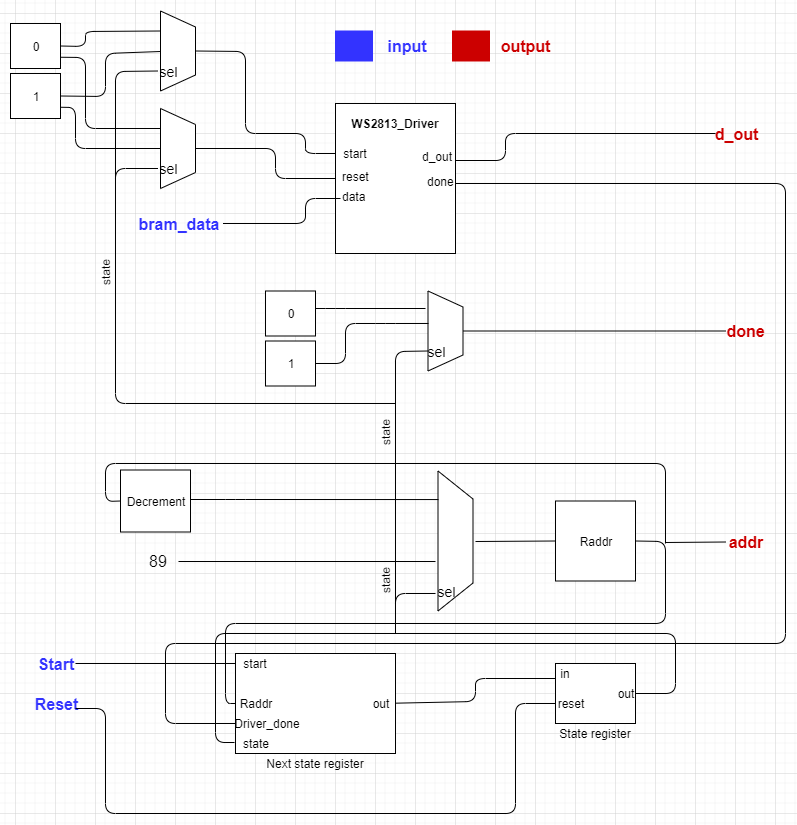
\includegraphics[scale=0.5]{WS2813_Controller_rtl.png}

\subsubsection{Állapotdiagram}

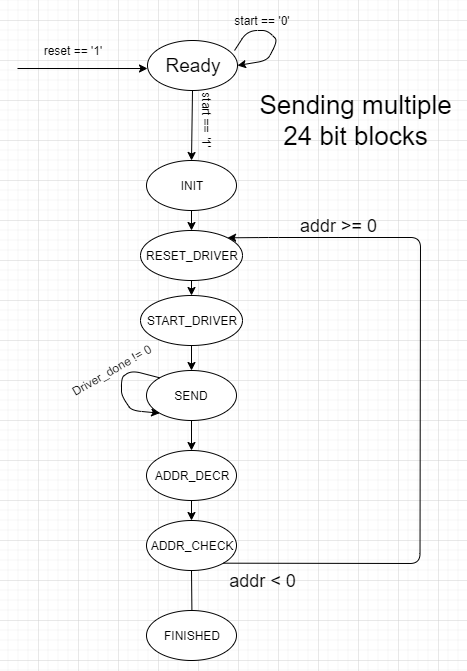
\includegraphics[scale=0.5]{WS2813_Controller_statedia.png}

\subsection{Alegységek}
\textbf{2019.10.14}
\begin{itemize}
\item Következő állapot regiszter \textbf{\textit{Next State Register}}
\item Állapot regiszter \textbf{\textit{State Register}}
\item Szín regiszter \textbf{\textit{Colour Register}}
\item Küldési logika regiszter \textbf{\textit{Transmission Logic Register}}
\end{itemize}

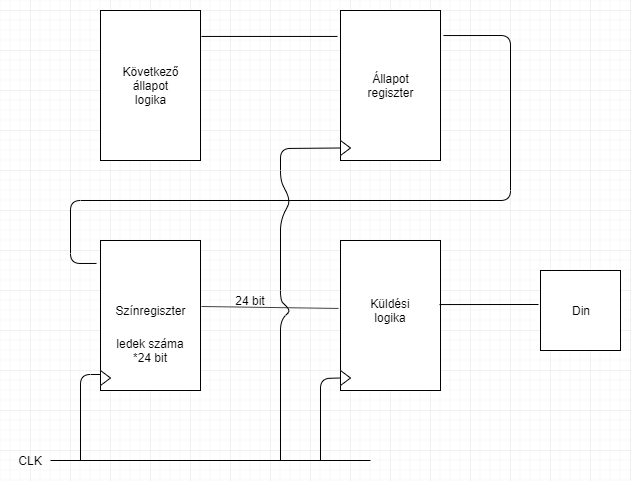
\includegraphics[scale=0.5]{tombvazlat.png}

\subsubsection{Küldési logika regiszter}

\noindent A küldési logika modul részletesebb lebontása: 

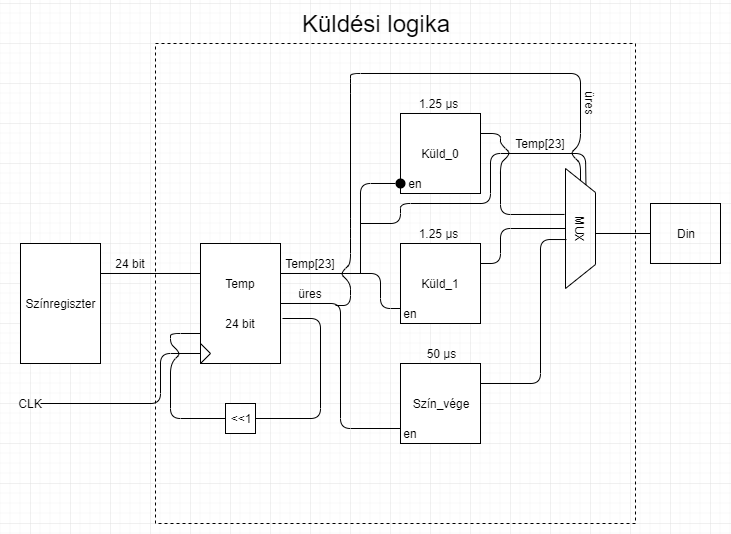
\includegraphics[scale=0.6]{kuldesi_logika.png}

\textbf{2019.10.28}

\indent Minden \textbf{led\_controll} modulhoz tartozik egy BRAM blokk és minden ilyen modul egy ledfűzért vezérel meg. Öt ilyen blokk megvezérel öt ledfűzért, ezáltal létrehozva a ledmátrixot.
Az órajel, start, reset, stop és data-rd jelek közösek minden modulnak.

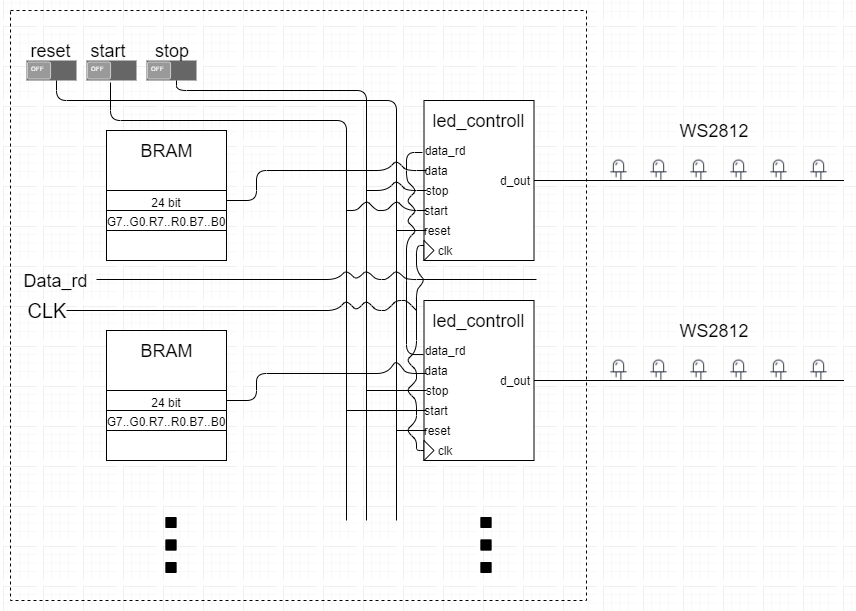
\includegraphics[scale=0.5]{tombvazlat2.png}

\subsection{Idődiagram}
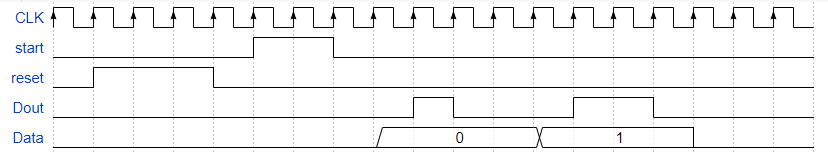
\includegraphics[scale=0.6]{general2.PNG}

\begin{itemize}
\item CLK: 100 MHz-es órajel
\item start: jel a folyamat elindításához
\item reset: jel a folyamat resetálásához
\item Dout: Egyszálú adatsín a LED-ekre.
\item Data: Kiírandó adat
\end{itemize}

\section{Szimuláció eredménye}
\subsection{WS2813\_Driver}

A \textbf{WS2813\_Driver} modul szimulációja alatt a következőkre figyeltem:
\begin{itemize}
	\item WS2813 egyszálú protokollja be van-e tartva
	\item A 24 bit-es blokkot sikerült-e legalább \SI{80}{\micro\second} alatt elküldeni (egy bitet elküldeni \SI{1.25}{\micro\second}, 24 bit-es blokk elküldése után min. \SI{50}{\micro\second}-ot kell várakozni) $1.25 * 24 + 50 = 80$ (\SI{}{\micro\second})
	\item A küldés befejezése után a \textbf{done} jel 1-esre lett-e állítva
\end{itemize}

A szimuláció során észrevevődött, hogy már az első kritérium nem teljesül:

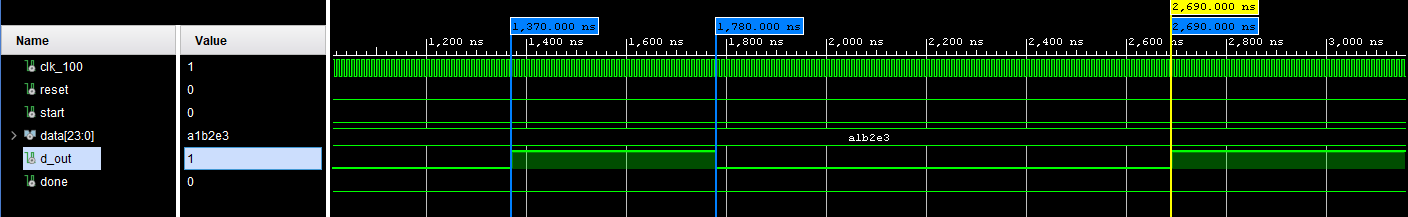
\includegraphics[scale=0.4]{driver_0_hibas.PNG}

Látható, hogy nullás küldése esetén a kimenet \SI{0.41}{\micro\second}-ot van magas feszűltésgen tartva \SI{0.45}{\micro\second} helyett és \SI{0.91}{\micro\second}-ot van
alacsony feszűltségen tartva, \SI{0.85}{\micro\second} helyett.

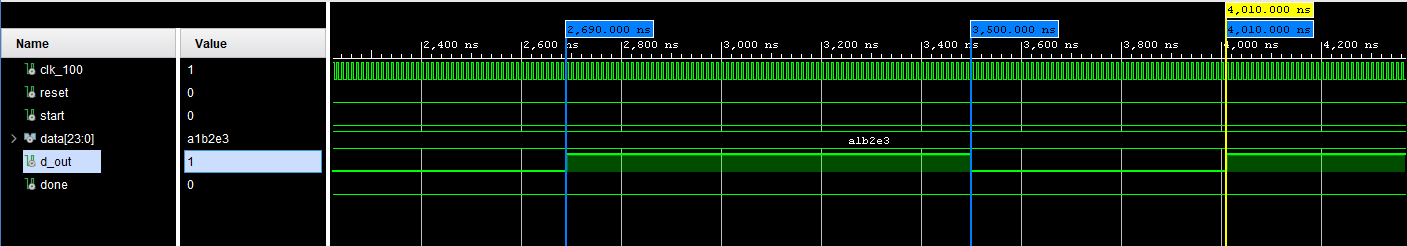
\includegraphics[scale=0.4]{driver_1_hibas.PNG}

Itt látható, hogy egyes küldése esetén a kimenet \SI{0.81}{\micro\second}-ot van magas feszűltésgen tartva \SI{0.8}{\micro\second} helyett és \SI{0.51}{\micro\second}-ot van
alacsony feszűltségen tartva, \SI{0.45}{\micro\second} helyett.

Ezt egyszerűen meg lehet oldani a ciklusszámok módosítása által.

Módosított ciklusszámok:

\begin{itemize}
\item Logikai 1-es
	\begin{itemize}
	\item 79 ciklus magas feszűltségen
	\item 39 ciklus alacsony feszűltségen
	\end{itemize}
\item Logikai 0-ás
	\begin{itemize}
	\item 39 ciklus magas feszűltségen
	\item 79 ciklus alacsony feszűltségen
	\end{itemize}
\end{itemize}

A frissített értékekkel a WS2813 protokollja már pontosan be van tartva.

Logikai egyesre:

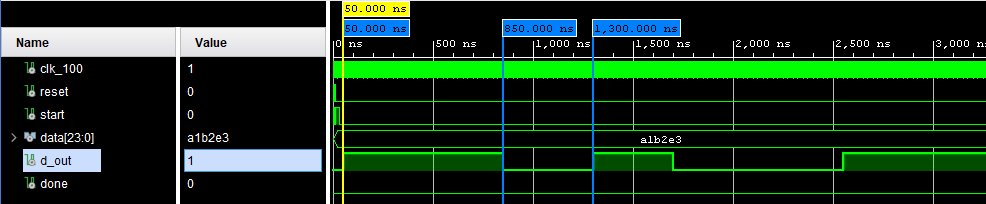
\includegraphics[scale=0.6]{driver_1_helyes.PNG}

Logikai nullásra:

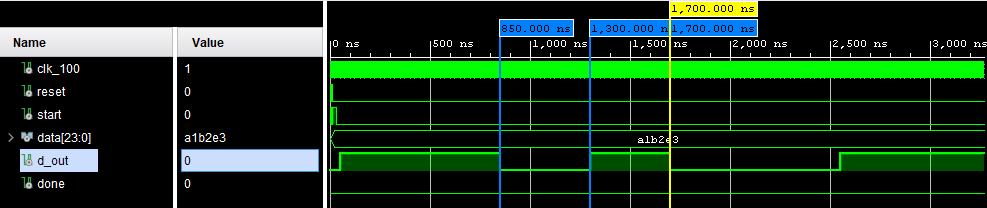
\includegraphics[scale=0.6]{driver_0_helyes.PNG}

A másik két követelmény is teljesül:

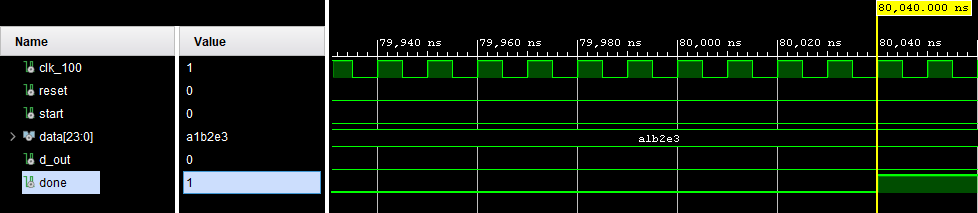
\includegraphics[scale=0.4]{driver_done.PNG}

A 24 bit-es blokk elküldése után a done jel egyesre lett állítva és \SI{80.04}{\micro\second} alatt sikerült az egész 24 bit-es blokkot elküldeni.


\subsection{BRAM memória}

A BRAM memóriának a használatát a következő két blogbejegyzés alapján tanultam meg: \href{http://vhdlguru.blogspot.com/2010/10/design-and-simulation-of-bram-using.html}{bram használata és tesztelése}
és \href{https://vhdlguru.blogspot.com/2010/10/how-to-use-coe-file-for-initializing.html}{BRAM feltöltése coefficient file használata által}.
A második blogbejegyzés alapján tanultam meg a BRAM memóriának a \textbf{coefficient} file alapján való feltöltését.
A BRAM memória szimulációja alatt azt értem, hogy megvizsgálom, hogy a BRAM memória helyesen fel lett töltve a \textbf{coefficient} file-ból.
A \textbf{coefficient} file:
\begin{verbatim}
	memory_initialization_radix=16;
	memory_initialization_vector=00A,00B,00C,00D,00E,00F,010,011,012,013,014,015,016,017,018,019;
\end{verbatim}

A szimuláció eredménye:

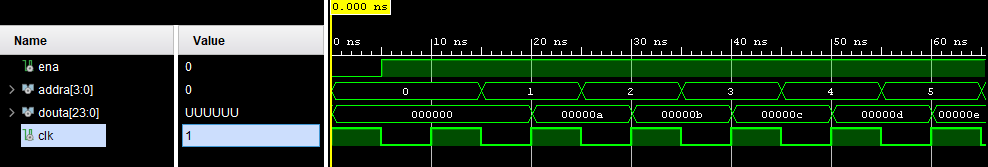
\includegraphics[scale=0.6]{bram_szimulacio.PNG}

Megfigyelésem alapján a generált BRAM modul felfutó órajelre olvassa be a következő címet, és ugyanúgy felfutó órajelre teszi ki az adatot a kimenetre, de csak egy egész órajellel a cím beolvasása után.


\section{Működés közbeni tesztelés - Integrated Logic Analyser}
\tab Működés közbeni tesztelés az FPGA-ba beépített ILA (Integrated Logic Analyser) és egy Tektronix logikai analizátorral volt elvégezve. A tesztelés beállításához (ILA) a TCL script-es megoldás\cite{brassai2018ukda_ila} volt felhasználva.
A Tektronix logikai analizátorral való teszteléssel a vezető tanár segített.

\subsection{WS2813\_Driver - ILA}

\tab Ennél a modulnál szükség van egy 24 bit-es bementre. Mivel annyi kapcsoló nem található a választott FPGA lapon, ezért a modul le lett egyszerűsítve, a tesztelés megkönnyebítéséért. 
24 bemenet helyett csak 4 lett felhasználva, ezek be is lettek konfigurálva az fpga négy kapcsolójára.

\tab Ezen kívül a done és a d\_out jelek egy-egy LED-re lettek kötve. A d\_out jelnek ledre való kötése később értelmetlennek bizonyult, mivel olyan gyors a váltakozás magas feszűltésgről alacsony feszűltségre
a küldés során, hogy a LED fel sem gyúl.

\tab A rendszer működés közbeni teszteléséhez szükséges volt egy trigger definiálásához: amikor a d\_out jel 1-esre vált, akkor kezdődjön a mintavételezés. Ez lehetővé teszi, hogy a küldés kezdetétől legyen a mintavételezés.

\tab FPGA állapota 0000 küldése esetén:

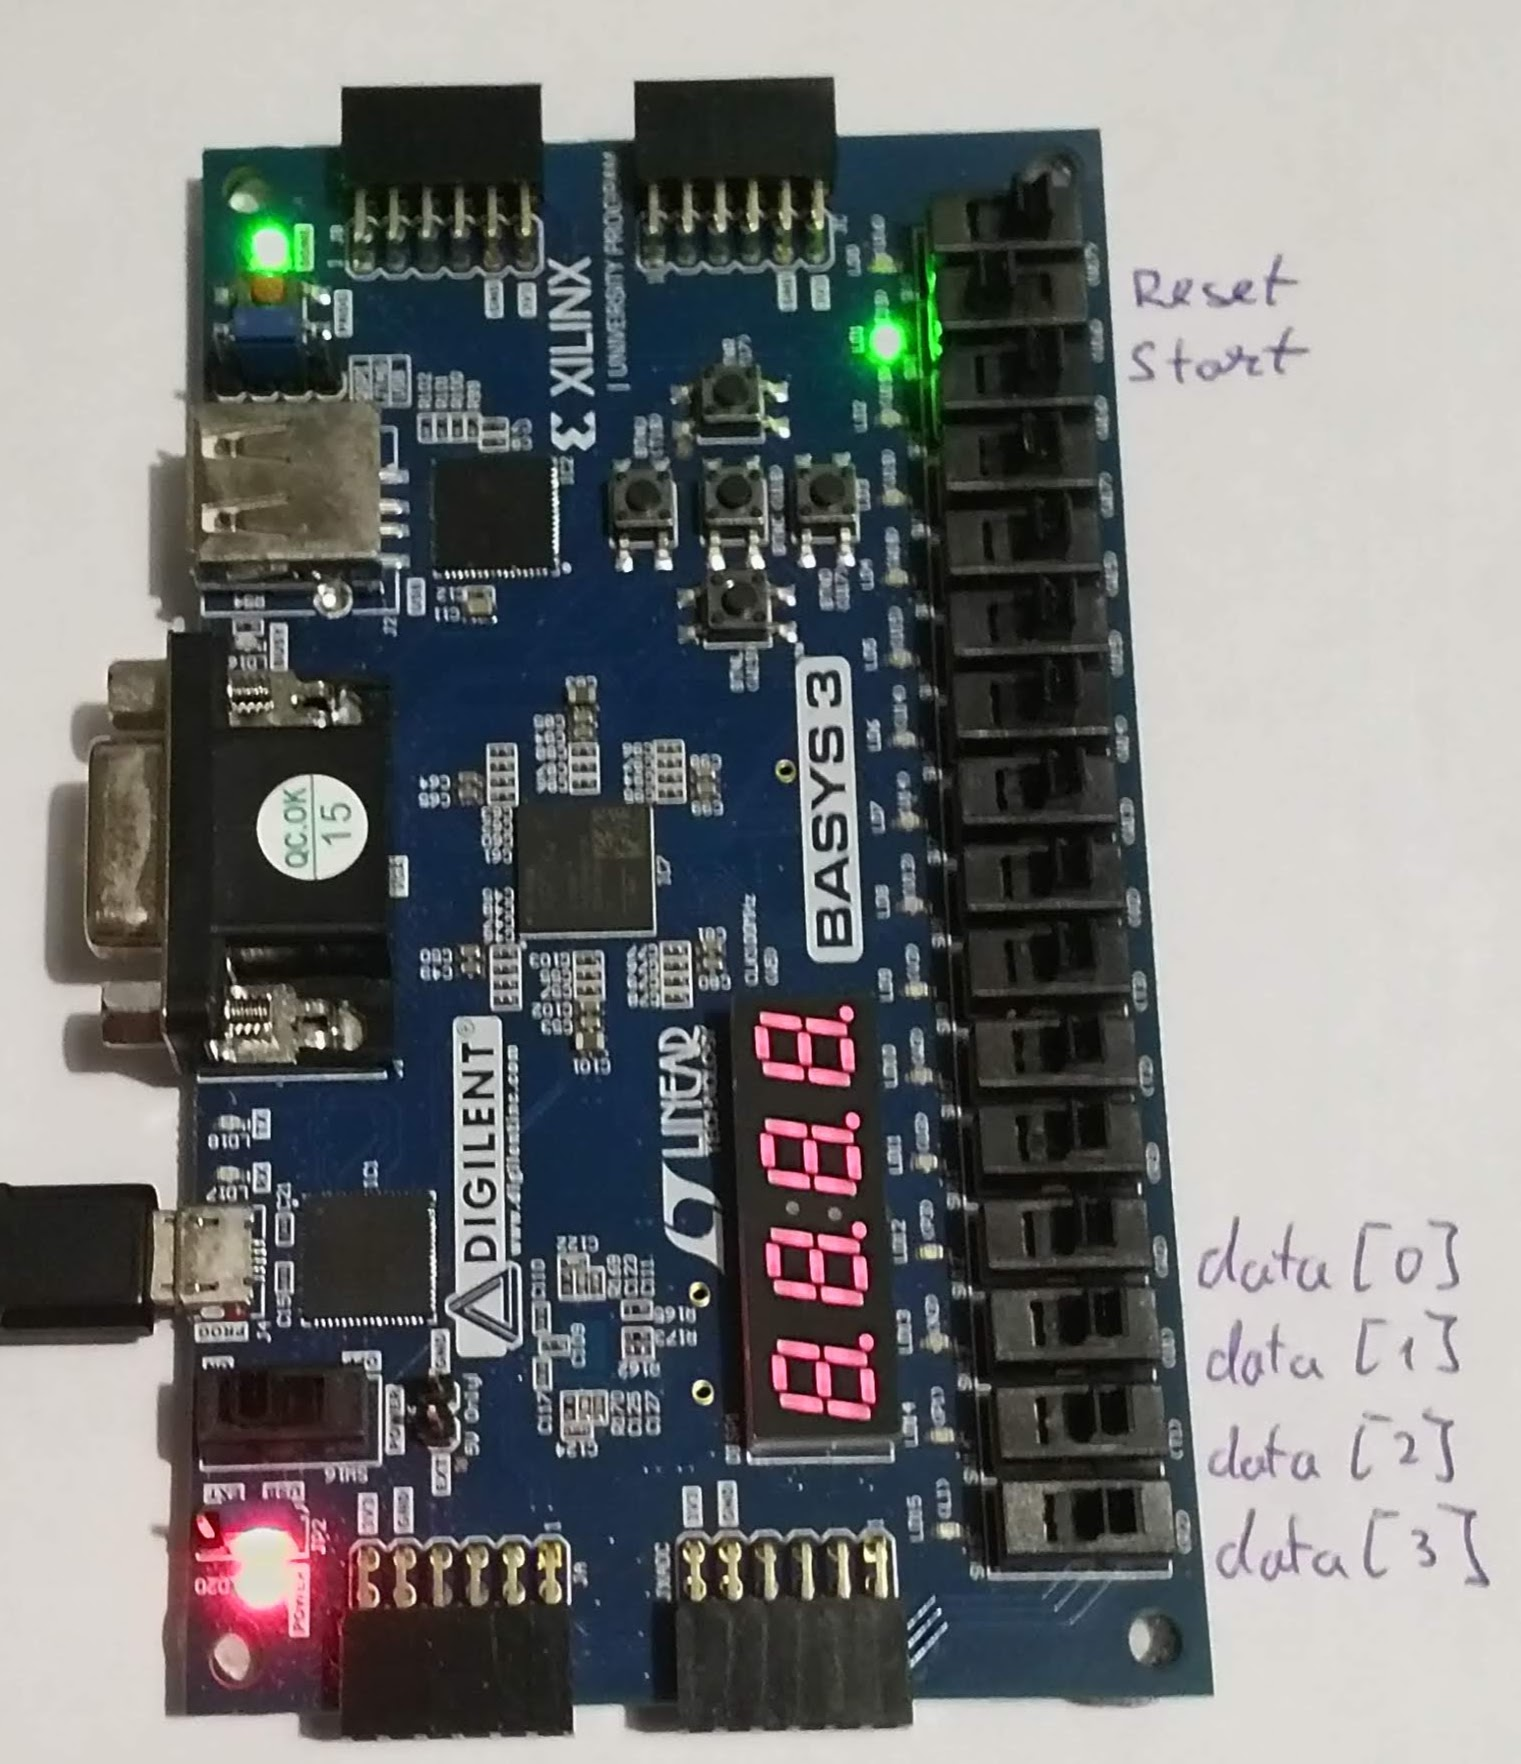
\includegraphics[scale=0.2]{fpga_0000.jpg}

\tab Jelek 0000 küldése esetén:

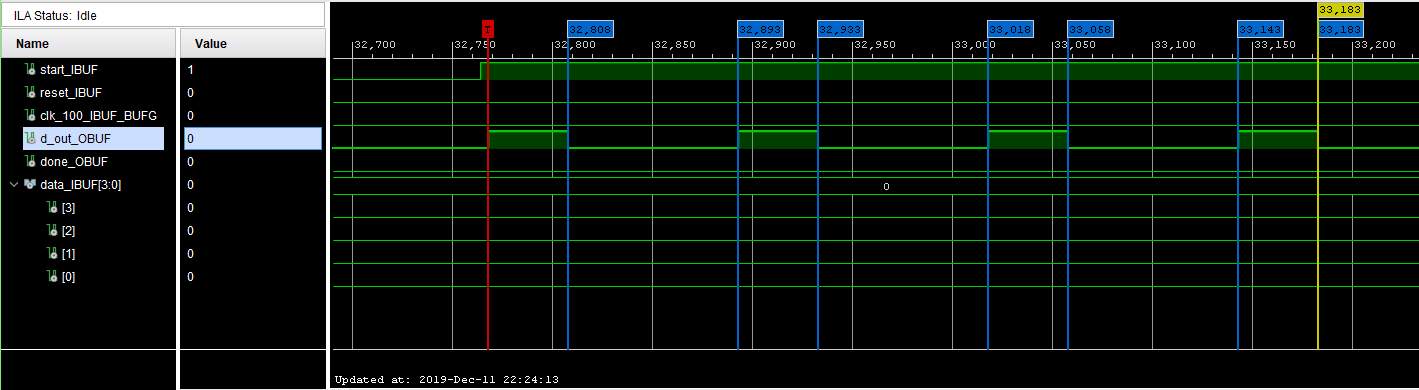
\includegraphics[scale=0.43]{ila_0000.PNG}

\tab Amint az FPGA-ról és a jelanalizálása közben is látható, az elküldött adat 0000. Ugyanakkor az is látható, hogy a d\_out jel annyi időt van magas és alacsony feszűltségen, amennyit a protokoll megkövetel.
Ezen a példán nem látszik, hogy a küldés az MSB-től (Most Significant Bit) lenne elkezdve. Ennek demonstrálásához egy "asszimetrikus" adat szükséges, mint például: 0010

\tab FGPA állapota 0010 küldése esetén:

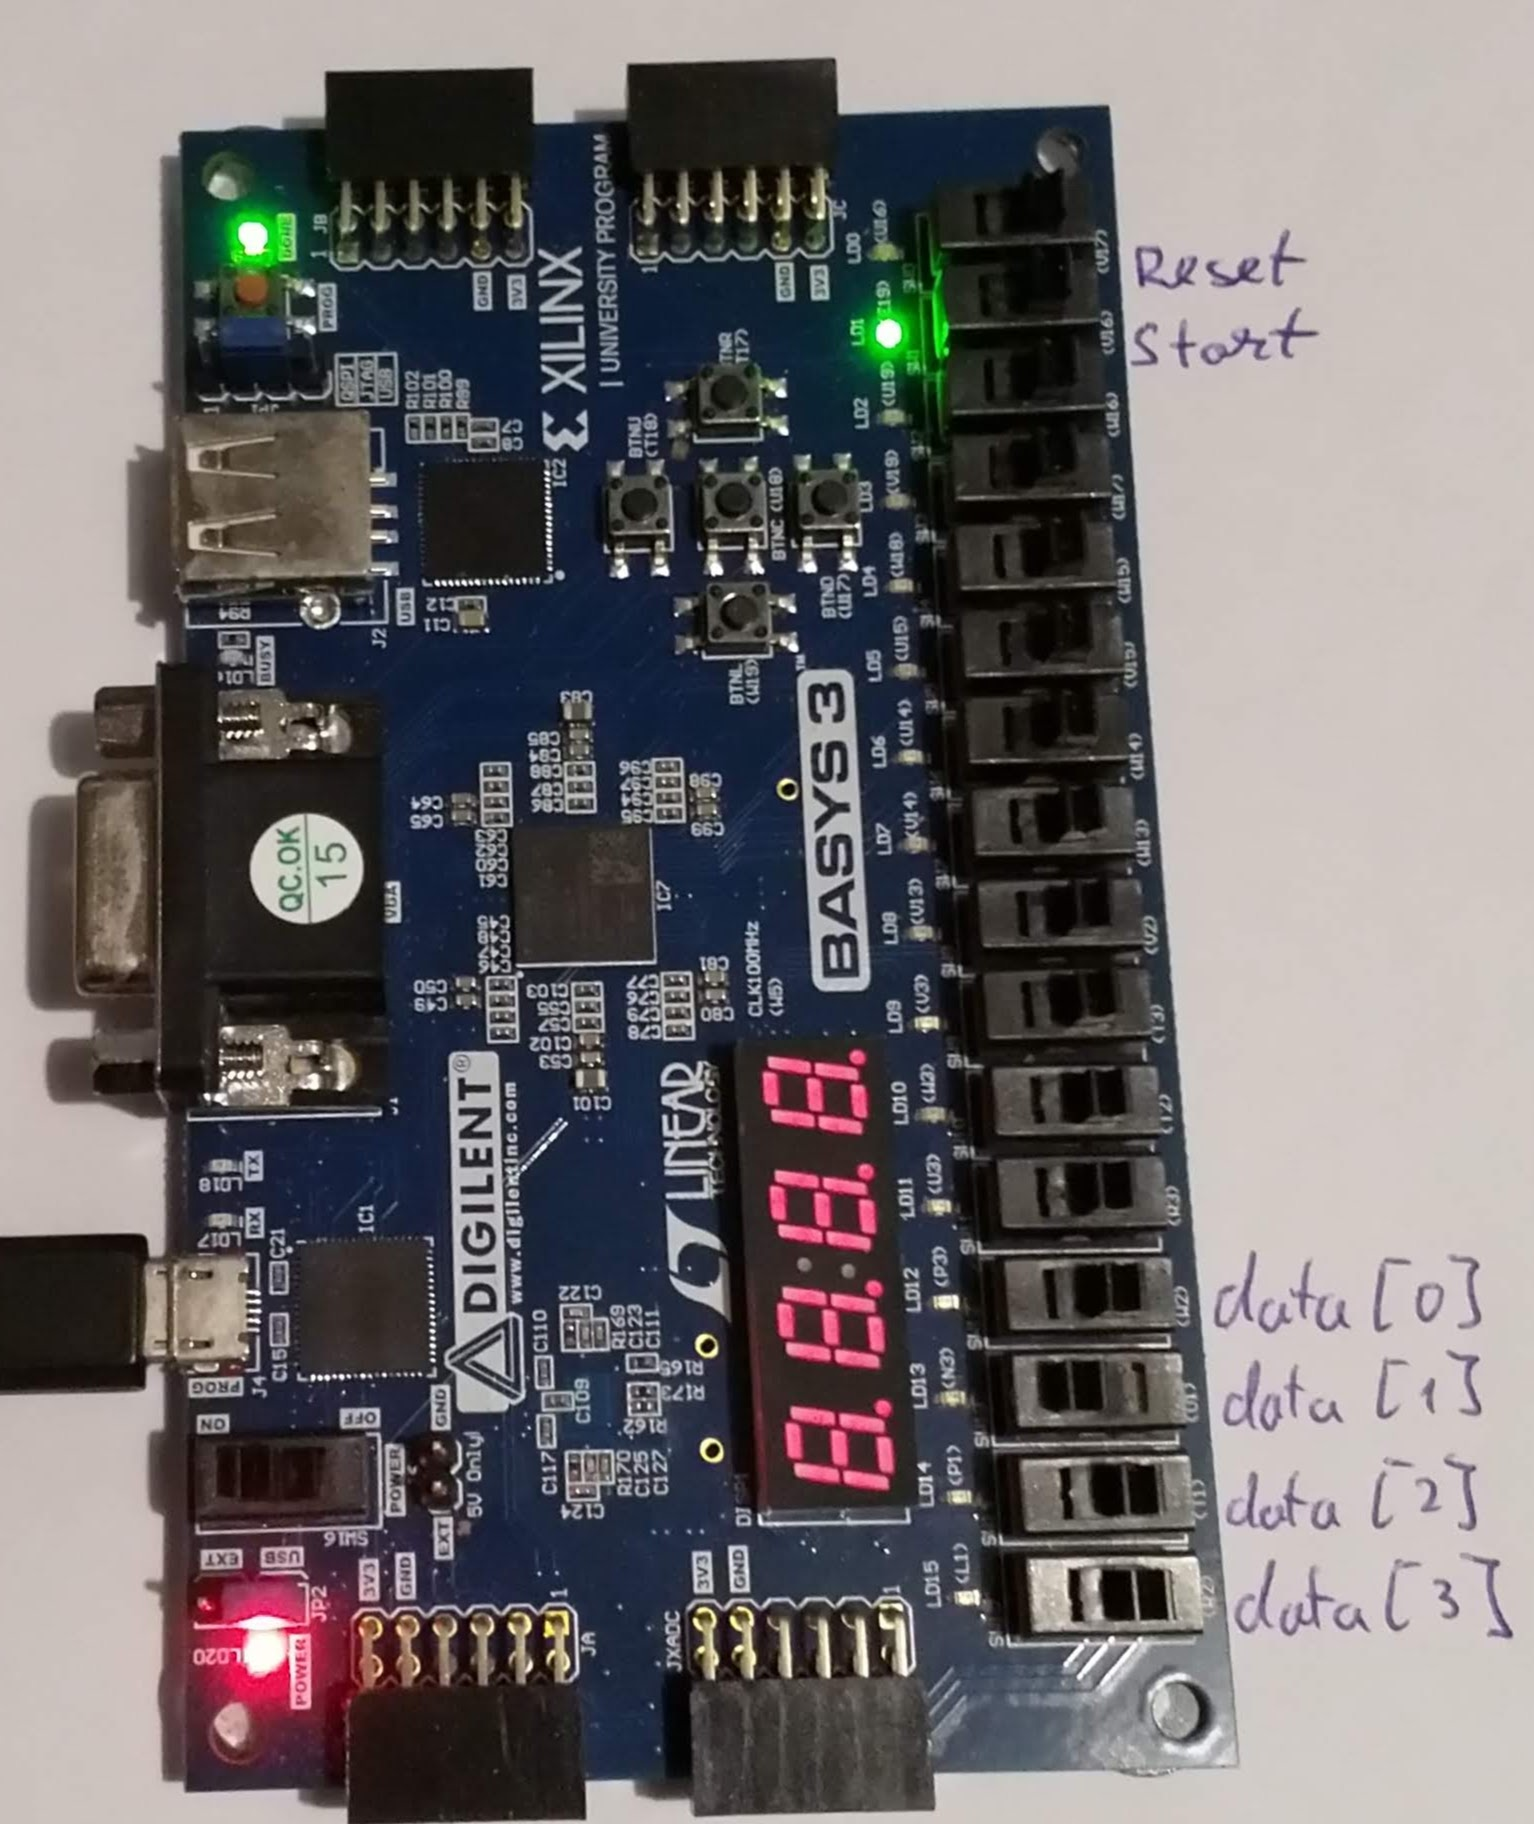
\includegraphics[scale=0.2]{fpga_0010.jpg}

\tab Jelek 0010 küldése esetén:

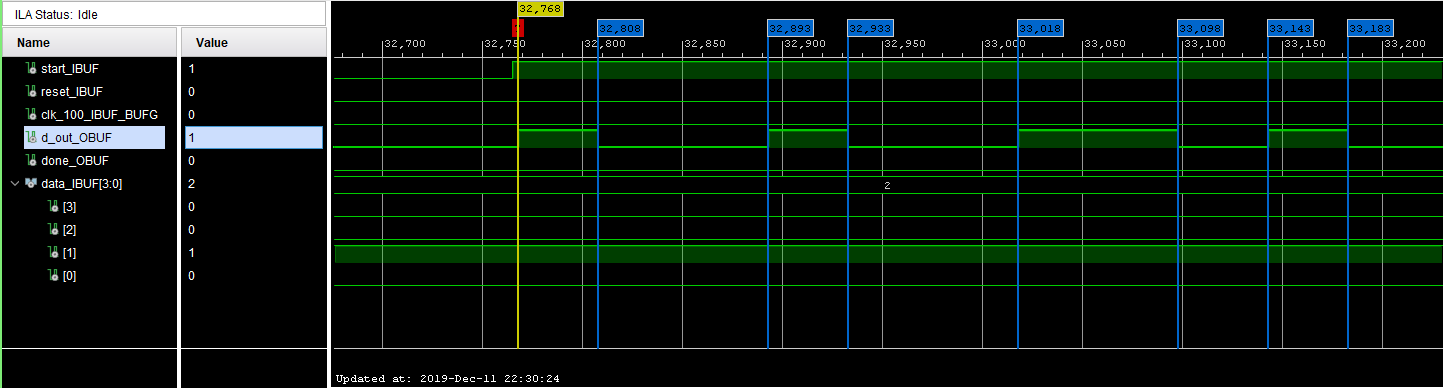
\includegraphics[scale=0.40]{ila_0010.PNG}

\tab Látható, hogy a küldés az MSB-től van elkezdve. Ugyanakkor az is megfigyelhető, hogy a WS2813 protokollja be van tartva.

\subsection{Teljes rendszer működés közbeni tesztelése - Tektronix logikai analizátor}

\tab A laborban található Tektronix logikai analizátorral sikerült elvégezni a működés közbeni tesztelést. A tesztelés alatt látható volt, hogy a 24 bit-es blokkok
helyesen küldődnek el, ugyanakkor az egyes bitek időzítése is helyesen történik.

Egy 24 bites blokk:

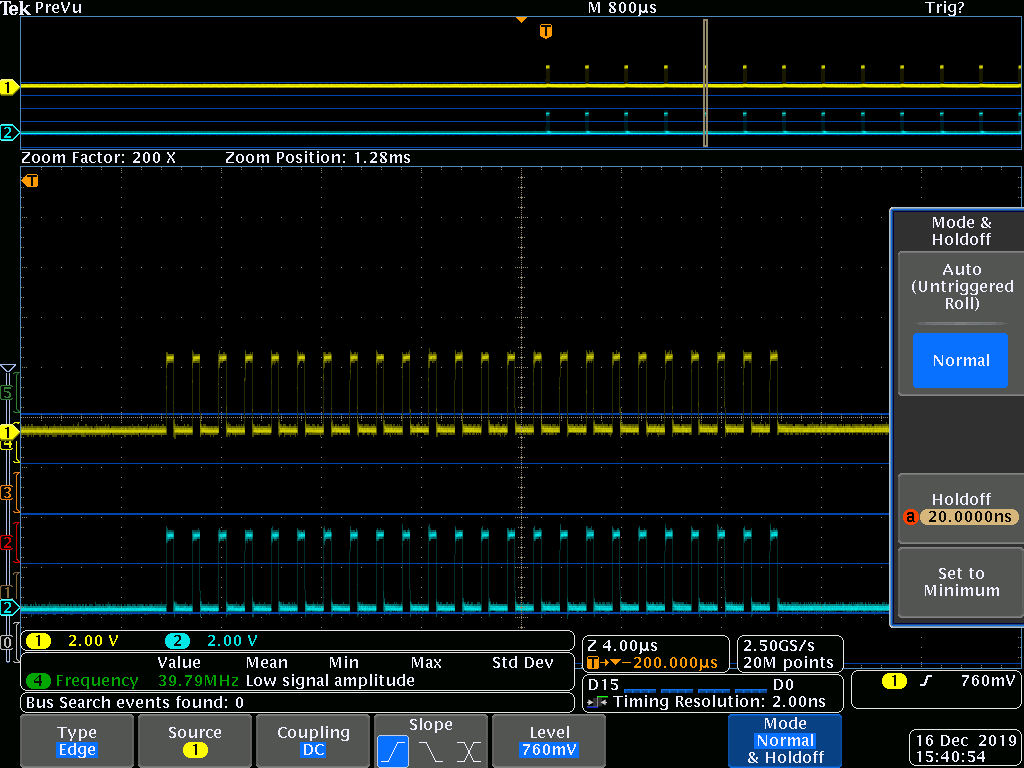
\includegraphics[scale=0.4]{tek00000.png}

24 bites blokkok küldése és a közöttük levő késleltetés

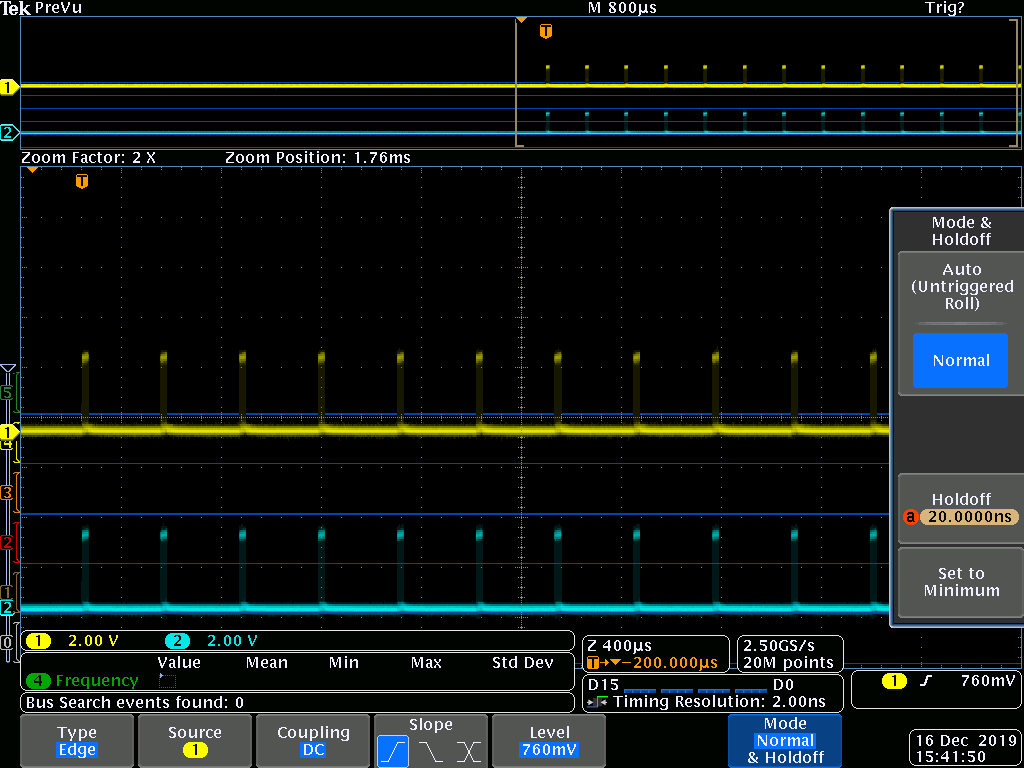
\includegraphics[scale=0.4]{tek00003.png}

\newpage
\bibliographystyle{ieeetr}
\bibliography{References}

\newpage
\appendix
\section{Tervezési lépések}
\subsection{Állapotok}

\subsubsection{Első iteráció - 2019.10.14}

\tab \textit{Ebben a fázisban még nem volt meg a megfelelő tudás a véges állapotú adatútas automatáról.
Itt a tervezés elnagyolva volt elvégezve, még nem volt kellőképpen átlátva a megoldandó probléma. A négy kontrolljel közül (start, reset, clear, stop)
csak kettő lett végül felhasználva: start és reset.}

Állapotok:
\begin{itemize}
\item READY
	\begin{itemize}
	\item Alap állapot 
	\item "reset" jel esetén ide kerül vissza az automata
	\end{itemize}
\item INIT
	\begin{itemize}
	\item minden LED-et kikapcsol (0x000000-t ír)
	\item "clear" jel esetén ide kerül az automata
	\end{itemize}
\item RENDER
	\begin{itemize}
	\item egyenként küldi a szín információt a LED-ekre
	\item annyiszor végződik el itt a művelet, ahány LED-ünk van
	\item "stop" jel esetén megáll a kiírás
	\end{itemize}
\item DISPLAY
	\item megtörtént a kiírás
\end{itemize}

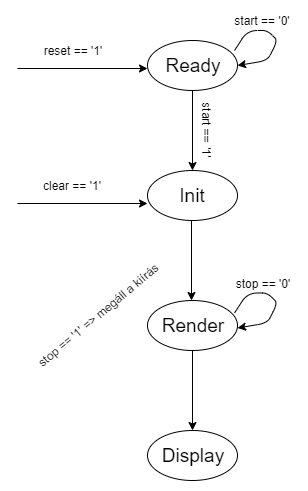
\includegraphics[scale=0.5]{allapotdiagram.png}

\subsubsection{Második iteráció - 2019.10.28}

\tab \textit{Ebben a fázisban kezdett kialakulni a szükséges tudás a feladat megoldásához, és a feladat is már jobban át volt látva. Itt már egy nagy modul helyett, két kisebb modulra van kigondolva
a feladat megoldása.}

\tab Állapotdiagram átírva úgy, hogy a küldési logikát is tartalmazza:

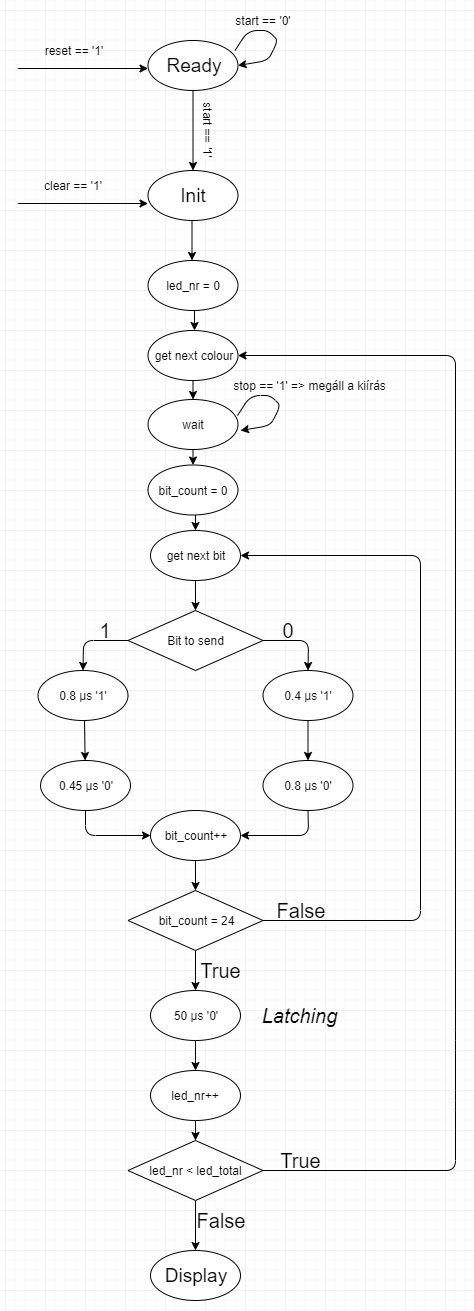
\includegraphics[scale=0.4]{allapotdiagram_2.png}

\tab \textit{Egy kisebb finomítás az állapotdiagramon. Itt már le van bontva részletesen az diagram RT műveletekre.}

\tab Állapotdiagram egy 90 LED-et vezérlő modulra

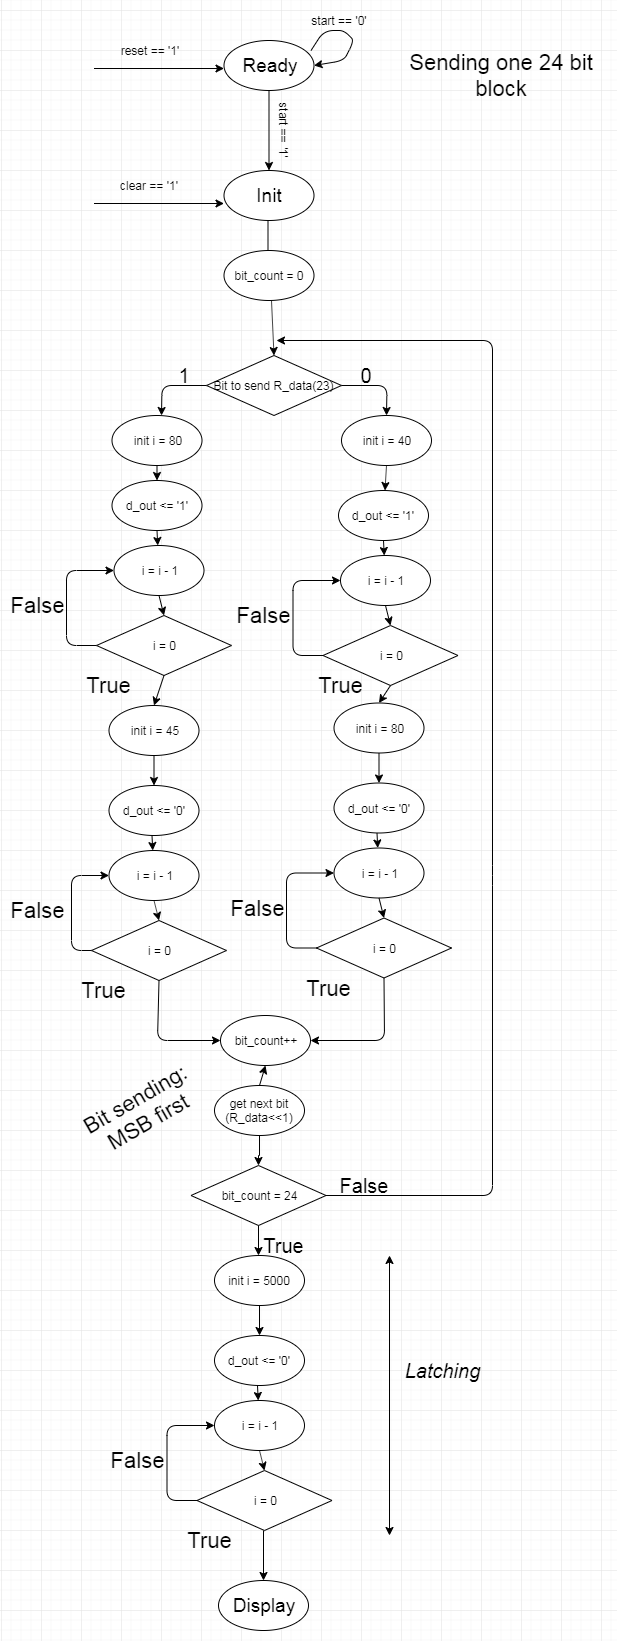
\includegraphics[scale=0.4]{allapotdiagram_3.png}


\subsection{Alegységek}

\subsubsection{Első iteráció - 2019.10.14}

\begin{itemize}
\item Következő állapot regiszter \textbf{\textit{Next State Register}}
\item Állapot regiszter \textbf{\textit{State Register}}
\item Szín regiszter \textbf{\textit{Colour Register}}
\item Küldési logika regiszter \textbf{\textit{Transmission Logic Register}}
\end{itemize}

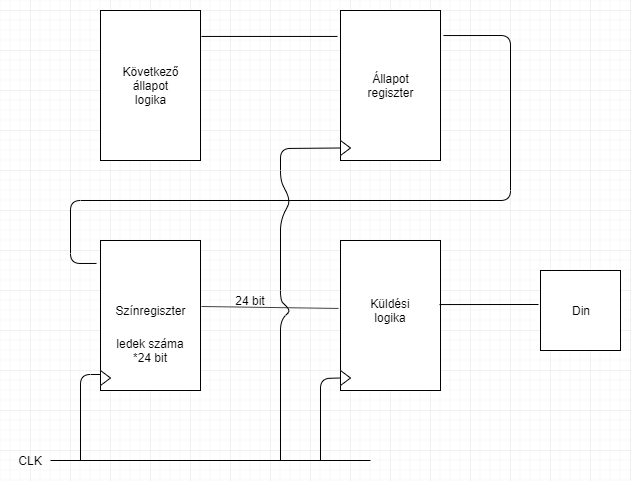
\includegraphics[scale=0.5]{tombvazlat.png}

\tab \textbf{Küldési logika regiszter}

\noindent A küldési logika modul részletesebb lebontása: 

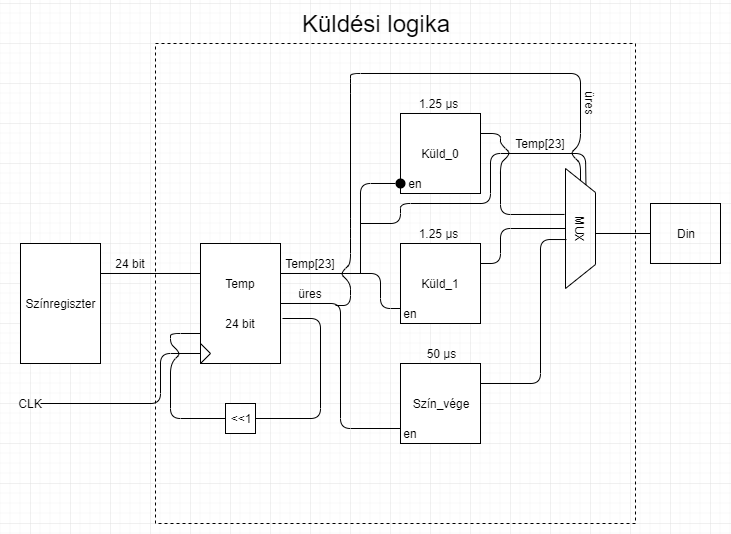
\includegraphics[scale=0.6]{kuldesi_logika.png}

\subsubsection{Második iteráció - 2019.10.28}

\tab Minden \textbf{led\_controll} modulhoz tartozik egy BRAM blokk és minden ilyen modul egy ledfűzért vezérel meg. Öt ilyen blokk megvezérel öt ledfűzért, ezáltal létrehozva a ledmátrixot.
Az órajel, start, reset, stop és data-rd jelek közösek minden modulnak.

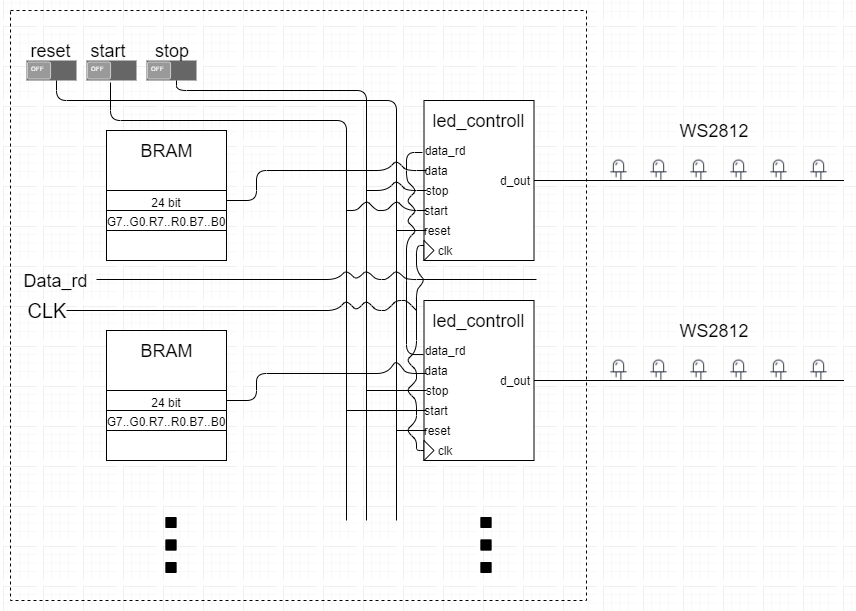
\includegraphics[scale=0.5]{tombvazlat2.png}


\subsection{Idődiagram}

\subsubsection{Első iteráció - 2019.10.26}

\tab \textit{Ebben a fázisban az volt az elgondolás, hogy a modul akkor olvassa be az adatot a \textbf{data} sínről, ha a \textbf{data\_rd} jel 1-es. Mint később kiderült,
erre nincs szükség.}

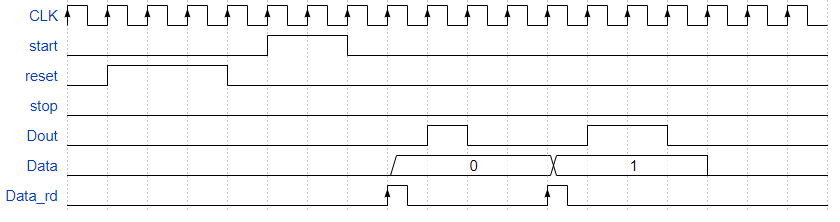
\includegraphics[scale=0.6]{general.PNG}

\begin{itemize}
\item CLK: 100 MHz-es órajel
\item start: jel a folyamat elindításához
\item reset: jel a folyamat resetálásához
\item stop: jel a kiírás megállításához. Csak két 24 bit-es blokk kiírása közben tudja megállítani a kiírást
\item Dout: Egyszálú adatsín a LED-ekre.
\item Data: Kiírandó adat, Data\_rd felmenő órajelére olvassa be az adatot.
\item Data\_rd: Aktiváló bit az adat beolvasására
\end{itemize}

\end{document}


